\documentclass{article}

\usepackage{graphicx, xcolor}
\usepackage{amsmath, amssymb}
\usepackage{float}
\usepackage[colorlinks=true,allcolors=blue]{hyperref}

\usepackage[margin=1in]{geometry}

\def\hwtitle{Homework 5: Linear Algebra}
\def\hwauthor{Caden Gobat}
\def\hwdate{\today}

\usepackage{fancyhdr}
\lhead{\hwauthor}
\chead{\hwtitle}
\rhead{\hwdate}
\lfoot{\hwauthor}
\cfoot{}
\rfoot{\thepage}
\renewcommand{\footrulewidth}{0.4pt}
\pagestyle{fancy}

\author{\hwauthor}
\title{\hwtitle}
\date{\hwdate}

\begin{document}

\maketitle
\thispagestyle{fancy}

\section{Introduction}

In this assignment, we employ the linear algebra technique of matrix-based Gaussian elimination to solve very large systems of equations that would be wildly unrealistic to undertake by hand.

\section{Results}

\bigskip
\noindent{\bf Question 1}
\medskip

The code-based numerical solution for the equivalent resistance between $(0,0)$ and $(1,1)$ on a $2\times2$ grid is 0.5 $\Omega$, if we take each individual resistor to have a value of 1 $\Omega$. To determine an analytical solution to this simple case, we recall the rules for summing resistors in series and in parallel:

\begin{gather*}
              \begin{aligned}
               R_{\text{s}} = \sum_{n} {R_n} \\ 
               \frac{1}{R_{\text{p}}} = \sum_{n} {\frac{1}{R_n}}
             \end{aligned}
\end{gather*}

Where $R_n$ is the value of each individual resistor. (Here, $R_n = 1\ \Omega\ \forall\ n$.) Because the resistors at the end of each column and row wrap back to the beginning, this grid simplifies to a circuit with two branches which are each made up of two pairs of parallel resistors in series with one another. Thus,
\begin{equation*}
    R_\text{eq} = \frac{1}{2\left(\frac{1}{1+1}+\frac{1}{1+1}\right)} = \frac{1}{2}\ \Omega
\end{equation*}
This agrees with the code's result.

\bigskip
\noindent{\bf Question 2}
\medskip

The equivalent resistance between the points $(1,1)$ and $(3,2)$ on a $5\times5$ grid is 0.68 $\Omega$. We get the exact same result for the resistance between the points $(0,0)$ and $(2,1)$ again due to the fact that the ``endpoint'' resistors wrap around and are thus not really endpoints at all, meaning that absolute positions are arbitrary---relative separations are all that matters in these problems.

\bigskip
\noindent{\bf Question 3}
\medskip

\begin{table}[H]
    \centering
    \begin{tabular}{c|c}
        $N$ & $R_\text{eq}$ \\
        \hline 
        10 & 0.748564 $\Omega$ \\
        20 & 0.767009 $\Omega$ \\
        30 & 0.770466 $\Omega$ \\
        40 & 0.771678 $\Omega$
    \end{tabular}
    \caption{Equivalent resistance between the nodes $(0,0)$ and $(1,2)$ on an $N\times N$ grid.}
    \label{tab:knightsjump}
\end{table}

\begin{figure}[H]
    \centering
    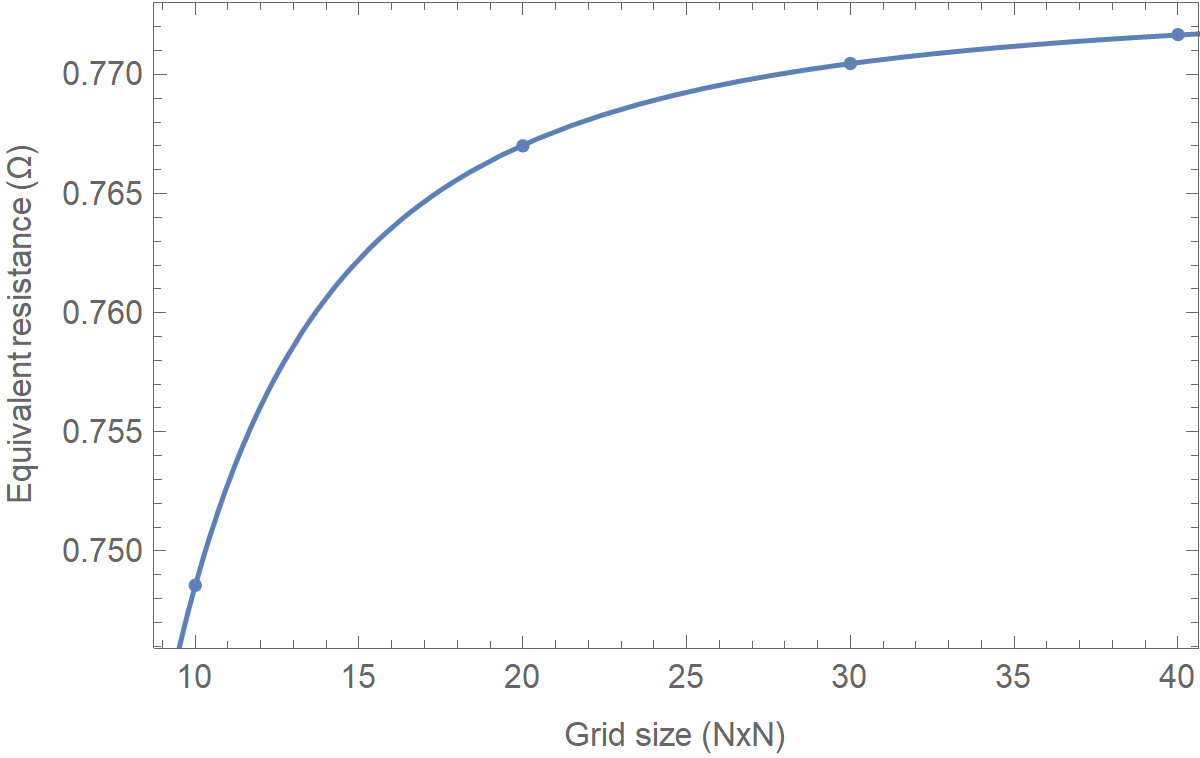
\includegraphics{homework5/3a.png}
    \caption{Equivalent resistances as a function of $N$ using a polynomial of the form $R_\text{eq}=a+b/N^2$. The optimized parameters are $a=0.7732$ and $b=-2.4641$. This model tells us that an infinite grid should have a resistance of 0.7732 $\Omega$ between these two points.}
    \label{fig:n2fit}
\end{figure}

\begin{figure}[H]
    \centering
    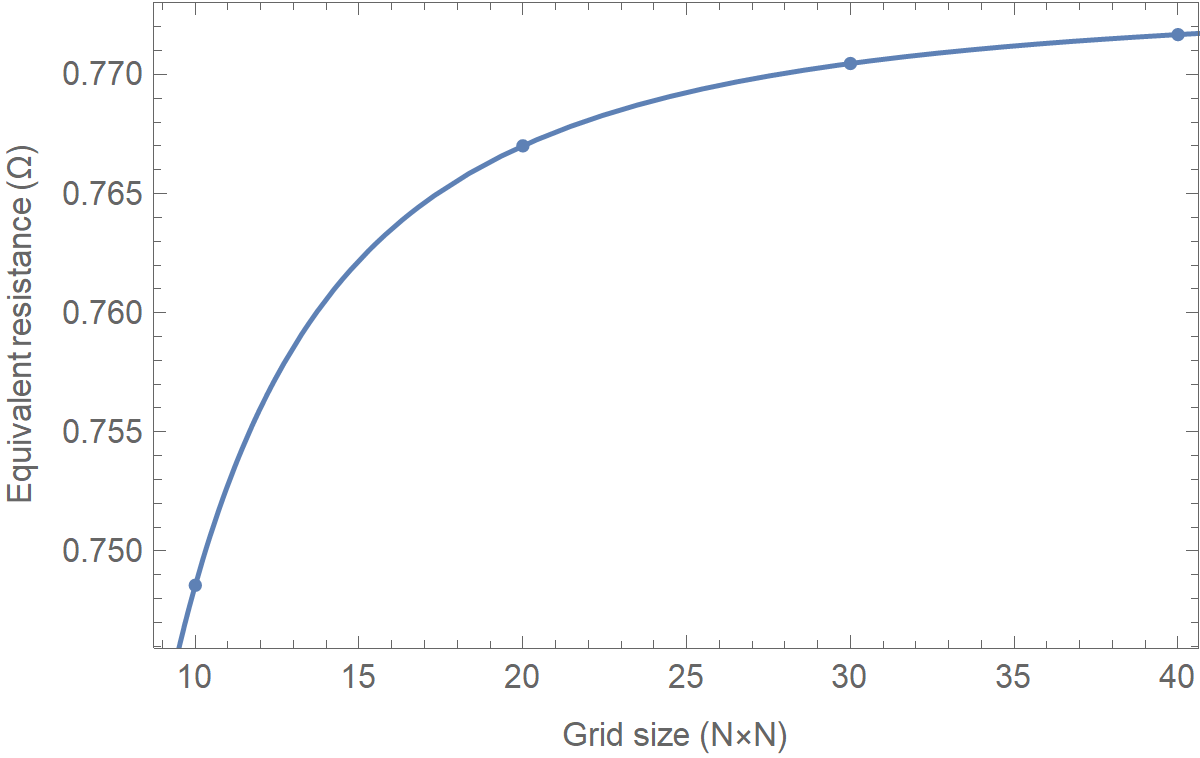
\includegraphics{homework5/3b.png}
    \caption{Equivalent resistances as a function of $N$ using a polynomial of the form $R_\text{eq}=a+b/N^2+c/N^4$. The optimized parameters are $a=0.7732$, $b=-2.5005$, and $c=3.2933$. This model tells us that an infinite grid should again have a resistance of 0.7732 $\Omega$ between these two points.}
    \label{fig:n4fit}
\end{figure}

The fits are both visually very close, and result in very similar results for $\displaystyle \lim_{N\to\infty}R_\text{eq}$. The second (fourth-order) function nominally allows for a closer fit, although theis raises the question as to whether this extra precision is warranted or whether it is an example of overfitting, given the already good fit granted by a function of order $N^{-2}$.

\bigskip
\noindent{\bf Question 4}
\medskip

\begin{table}[H]
    \centering
    \begin{tabular}{c|r}
        $N$ & CPU time \\
        \hline 
        10 & 0.030 s \\
        20 & 1.608 s \\
        30 & 18.108 s \\
        40 & 127.640 s
    \end{tabular}
    \caption{Computational times to determine the equivalent resistance between the nodes $(0,0)$ and $(1,2)$ with an $N\times N$ grid for various values of $N$.}
    \label{tab:timing}
\end{table}

The logarithmic slope (i.e., index of the power law) between the minimum and maximum points is 6.027. This tells us that the computational time scales as approximately $\mathcal{O}(N^6)$. A plot of the timing points and the fit through them using a function of the form $aN^6$ is shown in Fig.~\ref{fig:timing}. The best-fit value of $a$ here is approximately $3.1\cdot10^{-8}$.

\begin{figure}[H]
    \centering
    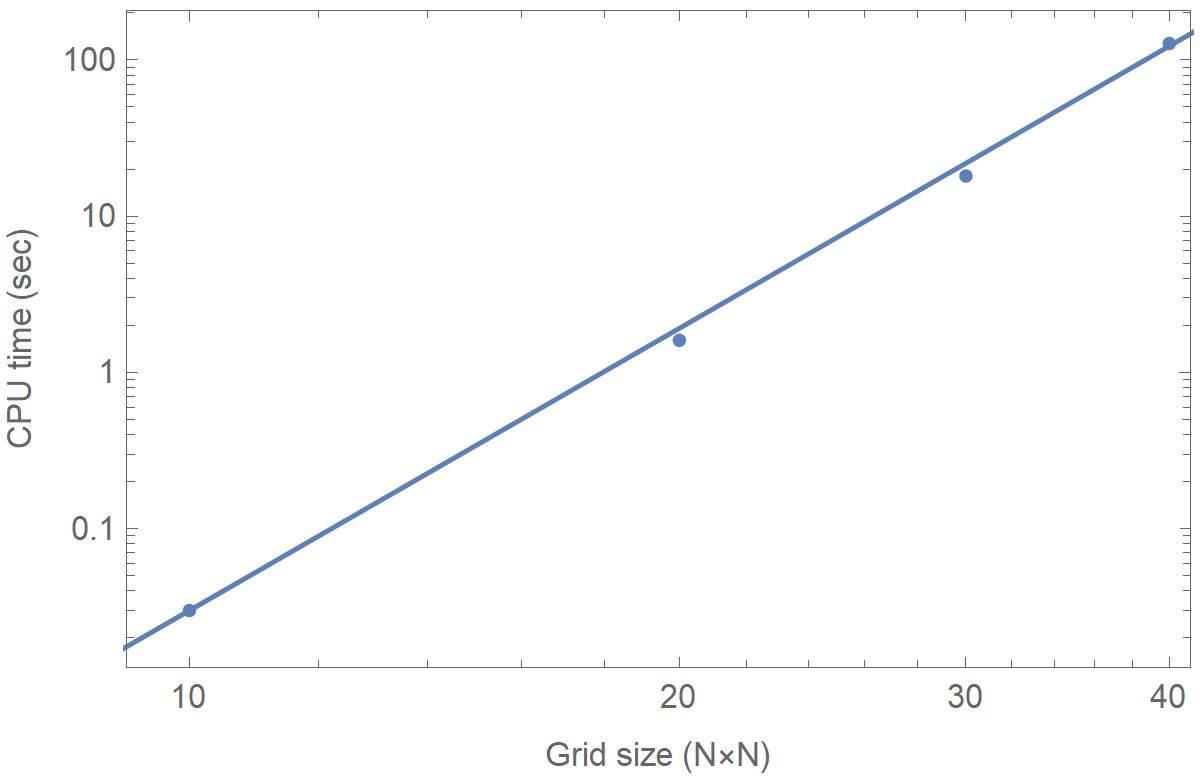
\includegraphics{homework5/time.png}
    \caption{CPU time used to calculate the equivalent resistances between the given points on a grid of dimension $N$. This relationship shows close adherence to a power law, as evidenced by the fact that it looks linear in log-space.}
    \label{fig:timing}
\end{figure}

\section{Conclusions}

The main challenge for me in this assignment was wrapping my head around the enumeration system for indexing the resistors and vertices on the grid. However, I eventually realized that because of the wrap-around nature of the setup, as long as every resistor and pair of nodes is accounted for, it actually does not matter how they are ordered in the backend of the code. Once the matrix is constructed, the Gaussian elimination algorithm does not care about the order of the equations.

With this conceptual barrier out of the way, I was able to fairly easily execute the rest of the tasks to solve the problems presented here, and having to code our own linear algebra routines certainly gave me a greater appreciation for the field as a whole.

\end{document}
